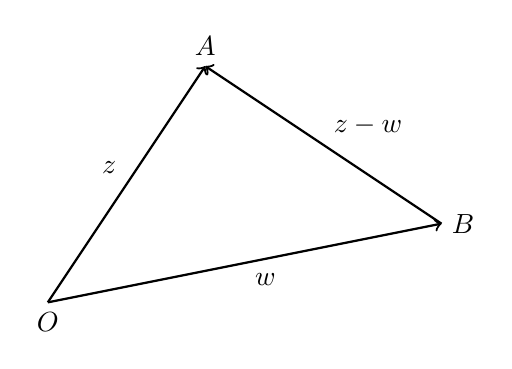
\begin{tikzpicture}[thick]
    \coordinate (O) at (0, 0);
    \coordinate (A) at (2, 3);
    \coordinate (B) at (5, 1);

    \draw[->] (O) -- (A) node[midway, above left] {\(z\)};
    \draw[->] (O) -- (B) node[midway, below right]  {\(w\)};
    \draw[->] (B) -- (A) node[midway, above right] {\(z - w\)};

    \node[below] at (O) {\(O\)};
    \node[above] at (A) {\(A\)};
    \node[right] at (B) {\(B\)};
\end{tikzpicture}